%%% LaTeX Template: Article/Thesis/etc. with colored headings and special fonts
%%%
%%% Source: http://www.howtotex.com/

\documentclass[12pt]{article}


\usepackage{apuntes-estilo}
\usepackage{fancyhdr,lastpage}
\usepackage{color,colortbl}
\usepackage{verbatim}

\def\maketitle{

% Titulo 
 \makeatletter
 {\color{bl} \centering \huge \sc \textbf{
  Aplicaciones Multimedia\\ 
\large \vspace*{-8pt} \color{black}Introducción a aplicaciones multimedia. 
 \vspace*{8pt} }\par}
 \makeatother

% Autor
\makeatletter
 {\centering \small 
 	Departamento de Ingeniería de Computadoras \\
 	Facultad de Informática - Universidad Nacional del Comahue \\
 	\vspace{20pt} }
 \makeatother

}

% Custom headers and footers
\fancyhf{} % clear all header and footer fields
\fancypagestyle{plain}{\fancyhf{}}
  	\pagestyle{fancy}
 	\lhead{\footnotesize Aplicaciones multimedia - Departamento de Ingeniería de Computadoras}
 	\rhead{\footnotesize \thepage\ }	% ''Page 1 of 2''

\def\ti#1#2{\texttt{#1} & #2 \\ }



\begin{document}

\thispagestyle{empty}
\maketitle
\setlength{\parindent}{0pt}

\section*{Introducción}

Para comprender el alcance de la palabra multimedia analizaremos distintas 
definiciones. Según la Real Academia Española, multimedia se refiere a un 
adjetivo que indica: ``que utiliza conjunta y simultáneamente diversos 
medios, como imágenes, sonidos y texto, en la transmisión de una 
información.''\cite{raemm}

\begin{center}
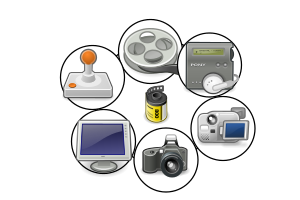
\includegraphics{multimedia.png}
\end{center}

Desde un punto de vista etimológico podemos decir que multimedia se 
refiere a: multi y media. Tal que multi se refiere a  muchos, y media a: 
substancia intermedia a través de la cual algo es transmitido o 
transportado. Un medio de comunicación masivo, tal como un periódico o 
la televisión.\cite{ramyer}

Estas definiciones nos das un primer acercamiento al alcance de la palabra
multimedia. Sin embargo, si nos preguntamos qué aspectos de este alcance 
serían importantes cubrir desde el punto de vista de {\it aplicaciones 
multimediales}, o desde la realidad de un administrador de sistemas y un 
entorno de trabajo convencional, como puede ser una oficina, todavía queda
mucho por aclarar. 

En este sentido la definición de Franklin Kuo, establece dos aspectos del
concepto de multimedia en los cuales haremos foco:

\begin{itemize}
\item Multimedia se refiere a la representación de medios mixtos de información
-texto, datos, imágenes, audio y video- como señales digitales. 
\item Comunicaciones multimedia, se refiere a la tecnología requerida para 
manipular, transmitir y controlar estas señales audiovisuales a través de un 
canal de comunicación.\cite{frankuo}
\end{itemize}

Los diferentes formatos de multimedia analógica o digital tienen la 
intención de mejorar la experiencia de los usuarios, por ejemplo para 
que la comunicación de la información sea más fácil y rápida. O, en 
el entretenimiento y el arte, para trascender la experiencia común.\cite{wikipmmes} 

Teniendo los dos aspectos mencionados por Kuo, si nos concentramos en contenidos 
multimedia dentro computadora aislada, es decir,  sin conexión a red (ya sea LAN o 
Internet), entonces nos enfocaremos por un lado en la representación y almacenamiento 
de datos multimediales, utilizando para ello los conocimientos previos 
adquiridos sobre formato interno de archivos regulares. Por otro lado, en 
las {\it aplicaciones multimedia} que nos permiten {\it generar} y manipular 
dichos contenidos localmente. 

Sin embargo, dado la expansión de Internet, y el frecuente desarrollo 
de redes de área local (LAN), debemos considerar el segundo aspecto mencionado
por Kuo referente a las {\it Comunicaciones multimediales}. La transmisión 
de datos multimediales sin dudas representa un desafío para los administradores
de sistemas en cuánto al análisis de recursos utilizados en dicha transmisión.
Una transmisión de video en vivo que no llega a tiempo a sus destinos, será 
una comunicación multimedial no exitosa, por lo que el análisis de los 
recursos necesarios se vuelve una tarea compleja e imprescindible en los 
sistemas modernos. 

Por último y nos menos importante, abordaremos brevemente los aspectos legales 
sobre la generación y transmisión de contenidos multimedia. En muchos casos,
hemos naturalizado el uso de imágenes, sonidos, textos y videos obtenidos 
desde Internet, sin prácticamente cuestionarnos acerca de la validez 
legal del uso que hacemos. Quizá es más evidente cuando se trata de 
películas o audio, ya que existen multiplicidad de campañas que, mal o 
bien, intentan introducir las consideraciones legales acerca de la descarga y 
reproducción de estos contenidos. Sin embargo, cuántos de nosotros nos 
preguntamos, por ejemplo al desarrollar el contenido de una wiki, si la 
imagen que acabamos de incorporar puede ocasionar un problema legal. 

En resumen, abordaremos multimedia siguiendo tres pilares:
\begin{itemize}
\item Aspectos estáticos: creación, reproducción (aplicaciones y formatos) y 
consumo de recursos, como ser almacenamiento y requisitos de procesamiento. 
\item Aspectos dinámicos: transmisión dentro de redes de área local (LAN) e 
Internet. 
\item Aspectos legales.  
\end{itemize}

\section*{Categorizaciones}

Desarrollaremos brevemente dos categorizaciones, ambas relacionadas a la 
percepción del usuario con respecto al contenido multimedia. En un caso 
nos referiremos a la interactividad del usuario; mientras que en el otro 
haremos referencia al componente temporal que puede o no afectar a la
reproducción de los contenidos. 

A la hora de evaluar contenidos multimedia, tendremos en cuenta entonces
por un lado los mecanismos de interacción (si los hubiere), y por otro 
cómo afecta el tiempo a la reproducción de elementos individuales. 

\subsection*{Interactividad}
En cuanto a la interacción que tiene el usuario con un contenido 
multimedial (como un todo, es decir un conjunto de elementos individuales
como texto, imagen, etc), podemos dividir dichos contenidos en: 
\begin{itemize}
\item Lineal: la reproducción de este tipo de contenidos progresa 
sin intervención del observador. Por ejemplo, un presentación cinematográfica.  
\item No lineal: en este caso, la interactividad es utilizada para 
controlar el progreso de la reproducción del contenido multimedial. Por 
ejemplo un video juego, una enciclopedia virtual en donde el observador
avanza a través de los contenidos que prefiere (ejemplo de hypermedia, 
wikipedia es una implementación posible), etc. 
\end{itemize}

\subsection*{Tipos de medios}
Por otra parte, teniendo en cuenta los elementos individuales que componen un 
contenido multimedia, podemos podemos distinguir dos grandes tipos de medios: 

\begin{itemize}
\item{Estáticos, medio discreto independiente del tiempo}
Dentro de esta clase encontramos a las imágenes y gráficos fijos, y texto. La información 
en este medio consiste exclusivamente de una secuencia de elementos individuales 
sin un componente de tiempo.
\item{Dinámicos, medio continuo dependiente del tiempo}
Aquí encontramos al sonido, animaciones y video. La información no sólo es 
expresada por su valor individual, sino que también por el momento 
de su ocurrencia.
\end{itemize}

Una aclaración importante acerca de esta calcificación es que la noción 
de {\it dependencia del tiempo} no tiene relación con la representación
del dato, en el sentido de que ambos medios, discretos y continuos, en su 
representación física puede no tener información acerca del componente 
temporal. El aspecto temporal en este caso, es más bien la percepción del 
que escucha u observa.\cite{ramyer}  

Claramente los medios continuos representarán un mayor desafío para el 
administrador a la hora de la transmisión a través de una red.   


\section*{Transmisión}


\section*{Aspectos Legales}

\begin{thebibliography}{1}

\bibitem{raemm}
Real Academia Española, \emph{Multimedia}.\hskip 1em plus
0.5em minus 0.4em\url{http://lema.rae.es/drae/?val=multimedia}

\bibitem{ramyer}
Ramesh Yerraballi, \emph{Multimedia Systems, Concepts Standards and 
Practice}.\hskip 1em plus  0.5em minus 0.4em
\url{http://users.ece.utexas.edu/~ryerraballi/MSB/Contents.html}

\bibitem{frankuo}
Franklin F. Kuo, J. Joaquin Garcia Luna-Aceves y Wolfgang Effelsberg. 
\emph{Multimedia Communications: Protocols and Applications}.\hskip 1em plus
  0.5em minus 0.4em\relax Publisher: Prentice Hall; ISBN-13: 978-0138569235  

\bibitem{wikipmmes}
Wikipedia en español. \emph{Multimedia}.\hskip 1em plus
  0.5em minus 0.4em\url{http://es.wikipedia.org/wiki/Multimedia}

\bibitem{wikipmmen}
Wikipedia en inglés. \emph{Multimedia}.\hskip 1em plus
  0.5em minus 0.4em\url{http://es.wikipedia.org/wiki/Multimedia}

\end{thebibliography}{1}

\section*{Licencia}
Copyright (C) 2014 Lechner Miriam.

Se concede autorización para copiar, distribuir y/o modificar este documento
bajo los términos de la Licencia Creative Commons Atribución-CompartirDerivadasIgual 3.0 Unported. 

http://creativecommons.org/licenses/by-sa/3.0/

\end{document}
